
\chapter{Motivation}
\section{Inspiration}
Inspired by the movie \textit{2001: A Space Odyssey} produced and directed by Stanley Kubrick, an adaption has been created by using povray. The adaption contains selected scenes of 5 minute clip on youtube.  With the exception of few scenes the cuts and scenes as well as the soundtrack are geared to the original video  \cite{EbClectic}.

\chapter{Models}
The whole short animation is created in povray. Everything but the starships (section \ref{imported_models}) has been created from scratch without using any tools.

\section{Imported Models} \label{imported_models}

We found the models of the Orion III Spaceplane and Space Station V by B.J. West with Textures by Michael Powell in the 2001: A Space Odyssey 3D Modelling Archiv \cite{Archive}.
Since both models were not available in a format directly usable with POV-Ray but \textit{3ds Max} (former called \textit{3D Studio Max}), we had to convert them from Autodesks proprietary format (.max) to the open Wavefront .obj format, which we then converted to POV-Ray code using PoseRay \cite{PoseRay}.

\section{Remarkable Models}
\subsection{Human} \label{human_model}
\subsection{Cabin}
\newpage
\subsection{Cockpit} \label{cockpit_model}
Inspired by the cockpit (figure \ref{cockpit_original}) shown in the movie, the cockpit in the adaption  is built completely from scratch using povray (figure \ref{cockpit_povray}). The starship \textit{Station} on this scene belongs to the imported models (section \ref{imported_models}).
The pilots are transformed models of the human (subsection \ref{human_model}).

\begin{figure}[ht]
	\centering
	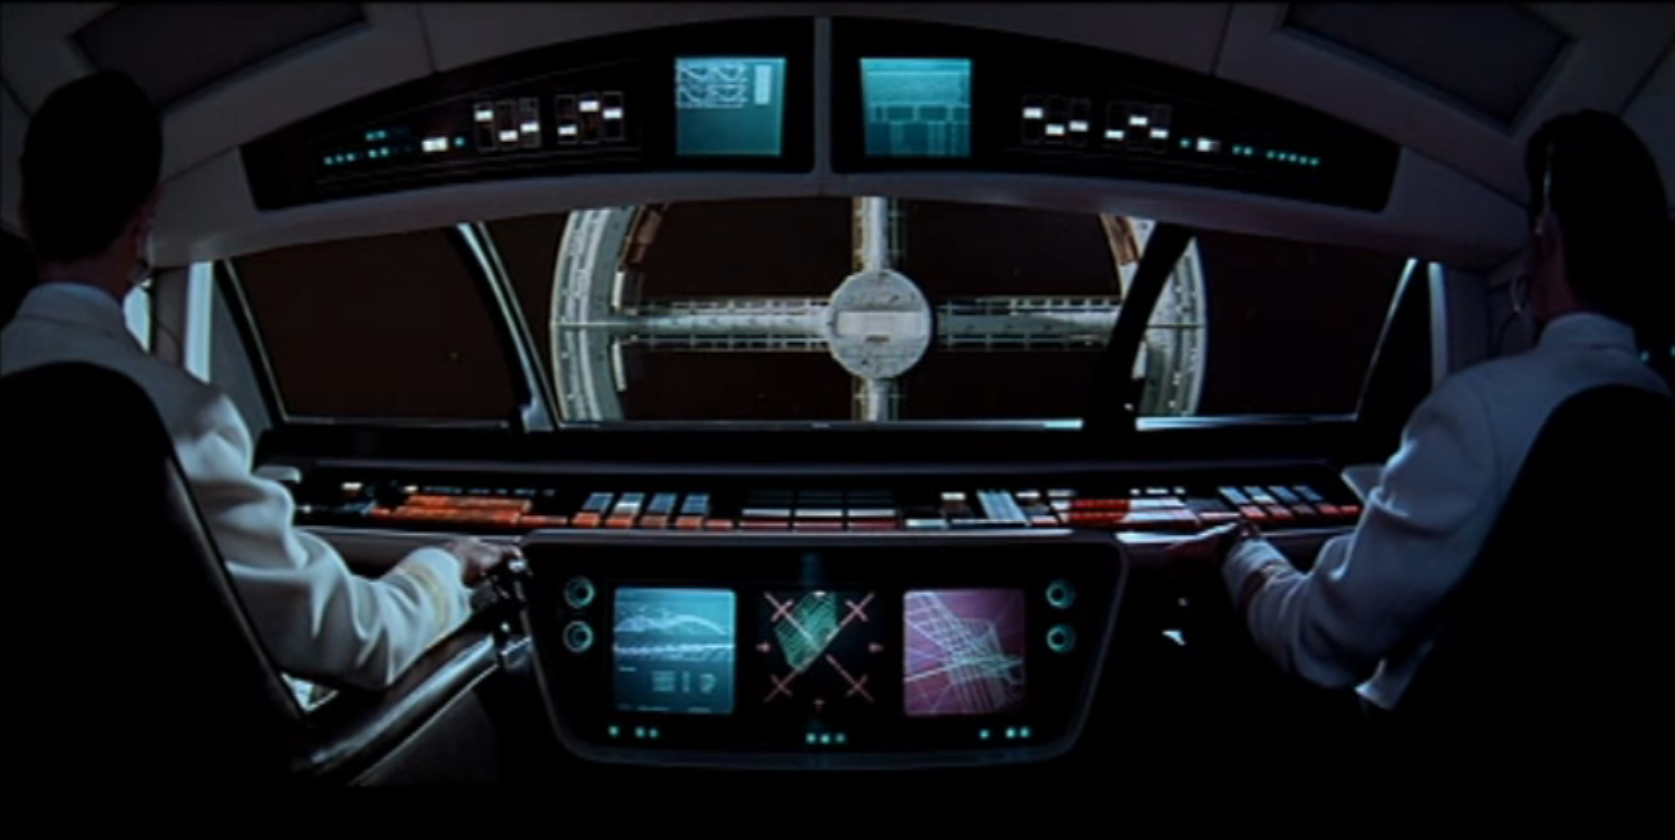
\includegraphics[width=0.85\textwidth]{images/original_cockpit.png}
	\caption{Cockpit of Starship \textit{Orion} taken from \textit{2001: A Space Odyssey}}
	\label{cockpit_original}
\end{figure}

\begin{figure}[ht]
	\centering
	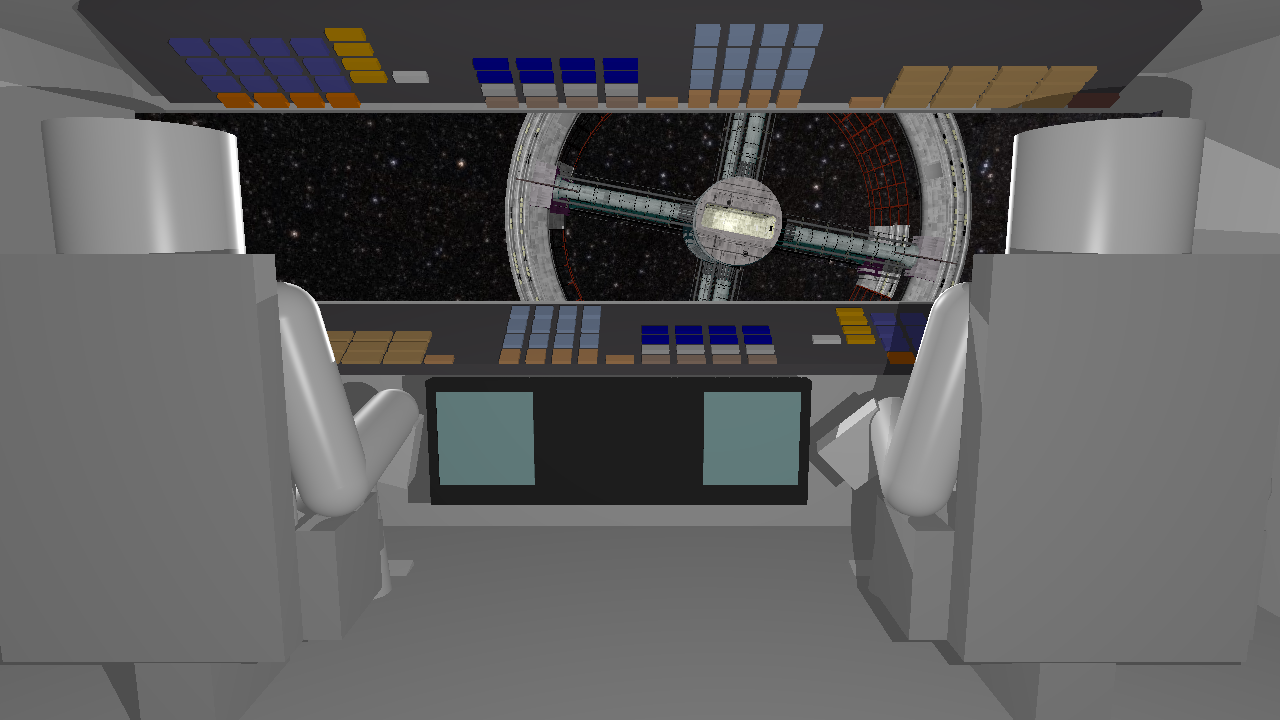
\includegraphics[width=0.85\textwidth]{images/scene19587.png}
	\caption{Cockpit of Starship \textit{Orion} built in povray.}
	\label{cockpit_povray}
\end{figure}

The associated povray script can be found on GitHub \cite{Quving}.

\newpage
\subsection{Planet}
As well as the cockpit (\ref{cockpit_model}) the planet shown in figure \ref{planet_original} has been recreated in povray (figure \ref{planet_povray}).
\begin{figure}[ht]
	\centering
	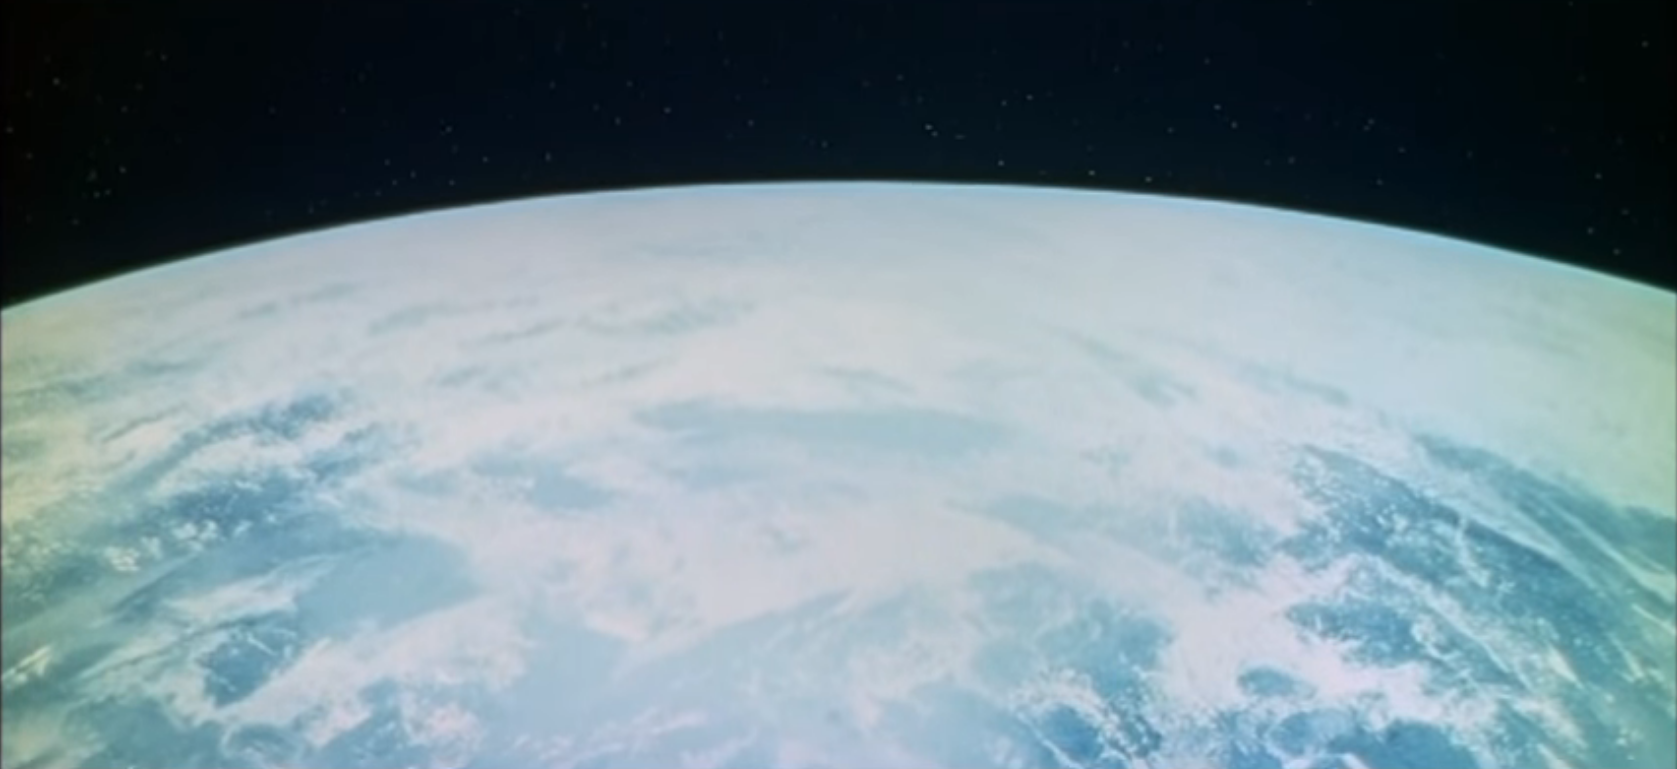
\includegraphics[width=0.85\textwidth]{images/original_planet.png}
	\caption{A picture of a planet taken from \textit{2001: A Space Odyssey}.}
	\label{planet_original}
\end{figure}

\begin{figure}[ht]
	\centering
	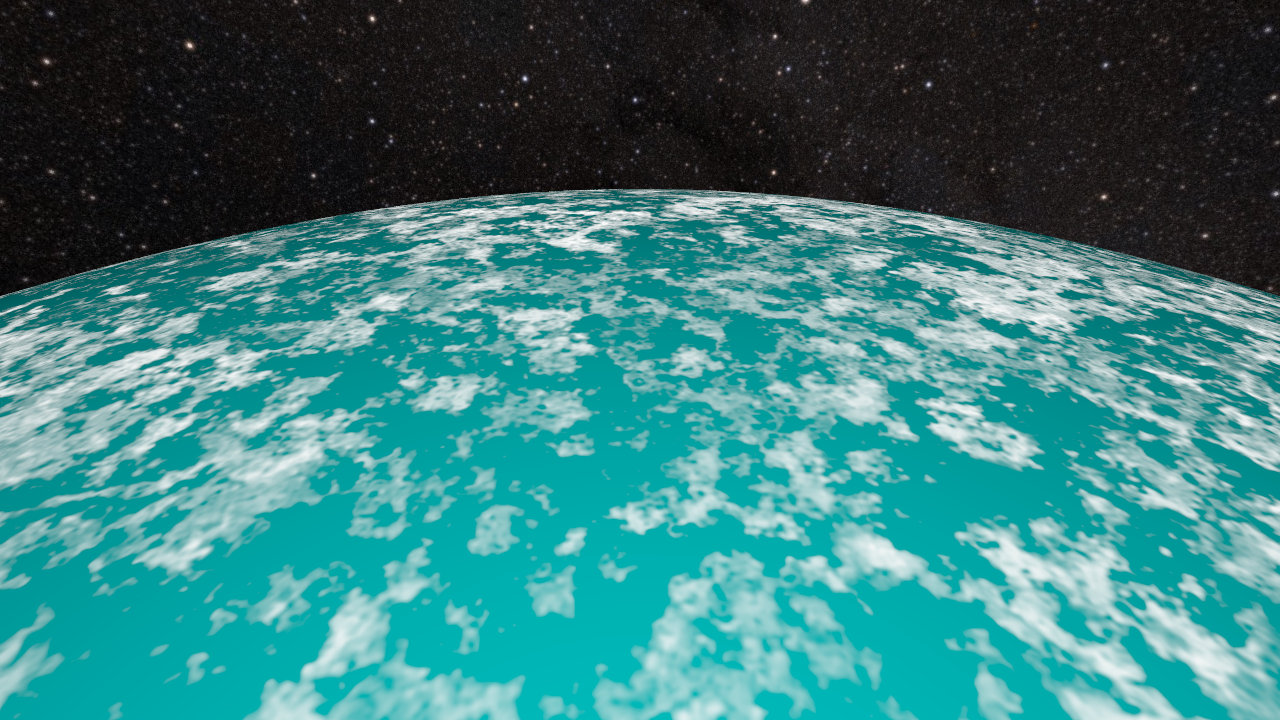
\includegraphics[width=0.85\textwidth]{images/scene04_05.jpg}
	\caption{This figure shows the result of a recreation of the above shown planet (\ref{planet_original}).}
	\label{planet_povray}
\end{figure}

The associated povray script can be found on GitHub \cite{Quving} and in the section \ref{povray_snippets}.

\newpage
\section{Povray Snippets} \label{povray_snippets}

\subsection{Planet}
\begin{lstlisting}
#declare PLANET = sphere {
	0, 5000
	rotate <clock*15, 0, 0>
	pigment { color rgb <0,0.75,0.75> }
	finish { ambient 0.00 diffuse 1}
	texture{
		pigment{
			bozo turbulence 0.075
			octaves 6  omega 0.7 lambda 2
			color_map {
				[0.0  color rgb <0.95, 0.95, 0.95> ]
				[0.05  color rgb <1, 1, 1>*1.25 ]
				[0.15 color rgb <0.85, 0.85, 0.85> ]
				[0.55 color rgbt <1, 1, 1, 1>*1 ]
				[1.0 color rgbt <1, 1, 1, 1>*1 ]
			}
		}
		finish { ambient 0 diffuse 1}
	}
}


\end{lstlisting}

\chapter{Production}

\section{Rendering} \label{rendering}
Once the frames are generated by povray. They are put together by using \textit{ffmpeg} to a video mp4 format. The following commandline renders frames with the prefix $scenex_XXX.png$ with 60 frame per second.

\begin{lstlisting}
$ ffmpeg -r 60 -start_number 1 -i scenex_%03d.png -c:v libx264 \
	-strict experimental -tune fastdecode -pix_fmt  \
	yuv420p -b:v 1500k out.mp4

\end{lstlisting}

\section{Post-Production}
Each scene is represented by a video obtained as above described (section \ref{rendering}). The final video and the soundtrack are cut by using \textit{Vegas Pro} \cite{VegasPro}.
